% ============================================================
%  CHAPITRE 1 : Fondements de la mécanique des fluides numérique
% ============================================================
\chapter{Fondements de la mécanique des fluides numérique}
\label{chap:fondements}

\section{Introduction}
\label{sec:introduction}

La modélisation constitue une représentation simplifiée d'un système complexe, visant à reproduire ses caractéristiques principales afin d'en faciliter l'analyse et la compréhension \cite{versteeg2007introduction}. Cette approche est essentielle pour appréhender des phénomènes naturels souvent régis par des interactions non-linéaires entre de nombreux paramètres, comme en météorologie, en aérodynamique ou en dynamique des fluides \cite{heller2011scale}. Face aux contraintes associées aux expérimentations physiques -- qu'elles soient coûteuses, dangereuses ou limitées par des effets d'échelle difficilement maîtrisables -- les modèles mathématiques et numériques s'imposent comme des alternatives incontournables \cite{ferziger2002computational}.

La Mécanique des Fluides Numérique (MFN), plus connue sous son acronyme anglais Computational Fluid Dynamics (CFD), constitue une branche spécifique de la mécanique des fluides dédiée à la simulation numérique du comportement des écoulements réels à partir des équations fondamentales, notamment les équations de Navier-Stokes \cite{roychowdhury2020computational}. Bien que ces équations soient connues depuis près de deux siècles, leur résolution analytique générale constitue encore aujourd'hui l'un des problèmes ouverts majeurs de la physique mathématique.

La CFD repose sur des méthodes issues de l'analyse numérique et des mathématiques appliquées, transformant un problème continu (espace et temps infinis) en un problème discret (nombre fini de points) résolvable par ordinateur \cite{patankar1980numerical}. Cette discrétisation permet d'approcher numériquement la solution des équations aux dérivées partielles qui régissent l'écoulement, offrant ainsi une vision approfondie des phénomènes physiques tout en assurant précision, réduction des coûts et sécurité \cite{tu2018computational}.

\section{Les équations de base de la mécanique des fluides}
\label{sec:equations_base}

L'analyse de tout problème en mécanique des fluides repose sur l'application des principes fondamentaux de conservation. La modélisation numérique des écoulements s'appuie sur la résolution d'équations de bilan traduisant trois principes essentiels : la conservation de la masse, la conservation de la quantité de mouvement et la conservation de l'énergie \cite{schlichting2016boundary}.

L'établissement de ces équations repose sur la définition d'un volume de contrôle, qui peut être fixe ou en mouvement selon l'approche adoptée. Deux descriptions sont couramment utilisées :
\begin{itemize}
    \item \textbf{L'approche lagrangienne} : le mouvement du fluide est décrit en suivant la trajectoire de particules fluides spécifiques. \item \textbf{L'approche eulérienne} : l'écoulement est analysé en observant les variations des grandeurs caractéristiques en des points fixes de l'espace \cite{anderson1995computational}. \end{itemize}

\begin{figure}[H]
    \centering
    \begin{minipage}{0.45\textwidth}
        \centering
        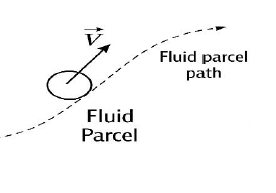
\includegraphics[width=\textwidth]{figures/figure1_2.png}
        \subcaption{Description lagrangienne}
        \label{fig:lagrangienne}
    \end{minipage}
    \hfill
    \begin{minipage}{0.45\textwidth}
        \centering
        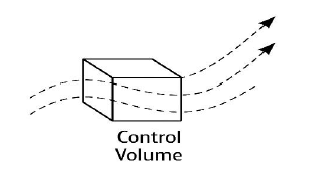
\includegraphics[width=\textwidth]{figures/figure1_3.png}
        \subcaption{Description eulérienne}
        \label{fig:eulerienne}
    \end{minipage}
    \caption{Représentations des approches lagrangienne et eulérienne en mécanique des fluides.}
    \label{fig:approches_lagrangienne_eulerienne}
\end{figure}

\subsection{L'équation de continuité}
\label{subsec:continuite}

L'équation de continuité traduit le principe de conservation de la masse, stipulant que le taux de changement de la masse du système dans le temps est nul \cite{batchelor1967introduction}. Pour un volume de contrôle fixe, la forme intégrale s'écrit :

\begin{equation}
\frac{\partial}{\partial t} \int_{V_c} \rho \, d\Omega + \int_{S_c} \rho \, \vec{V} \cdot \vec{n} \, dS = 0
\label{eq:continuite_integrale}
\end{equation}
\begin{itemize}
    \item[--] \(t\) : le temps
    \item[--] \(V_c\) : le volume de contrôle
    \item[--] \(\rho\) : la masse volumique du fluide \([kg/m^3]\)
    \item[--] \(\Omega\) : le domaine du volume de contrôle
    \item[--] \(S_c\) : la surface de contrôle (frontière du volume de contrôle)
    \item[--] \(\vec{V}\) : le vecteur vitesse du fluide \([m/s]\)
    \item[--] \(\vec{n}\) : le vecteur unitaire normal à la surface \(S_c\), orienté vers l'extérieur
\end{itemize}

Cette équation indique que la somme de la variation temporelle de la masse contenue dans le volume de contrôle et du flux massique à travers sa surface est nulle, comme illustré par le volume de contrôle fixe représenté à la Figure~\ref{fig:volume_controle_fixe}. Par application de la formule de divergence sur un volume élémentaire infinitésimal (Figure~\ref{fig:volume_elementaire}), on obtient la forme locale de l'équation de continuité : \cite{panton2013incompressible}

\begin{equation}
\frac{\partial \rho}{\partial t} + \nabla \cdot (\rho \vec{V}) = 0
\label{eq:continuite_locale}
\end{equation}

Pour un fluide incompressible, hypothèse valable pour l'eau dans la plupart des applications hydrauliques, la masse volumique reste constante, ce qui simplifie l'équation à :

\begin{equation}
\nabla \cdot \vec{V} = 0
\label{eq:continuite_incompressible}
\end{equation}

\begin{figure}[H]
    \centering
    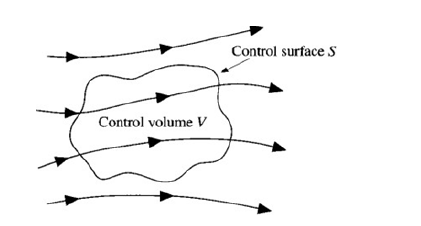
\includegraphics[width=0.6\textwidth]{figures/figure1_4.png}
    \caption{Volume de contrôle fixe traversé par le fluide en mouvement.}
    \label{fig:volume_controle_fixe}
\end{figure}

\begin{figure}[H]
    \centering
    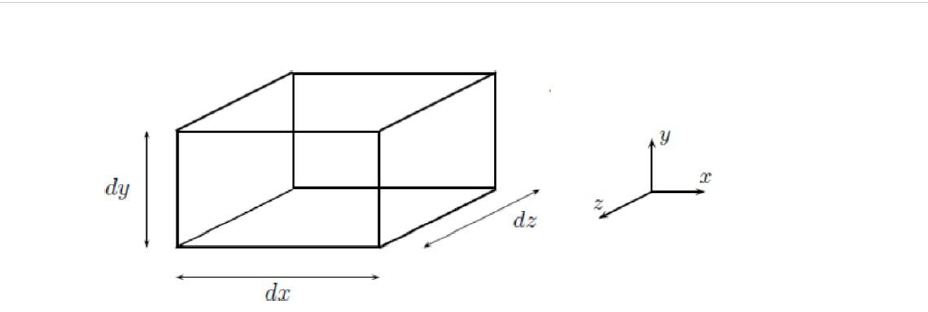
\includegraphics[width=0.6\textwidth]{figures/figure1_5.png}
    \caption{Volume élémentaire fixe pour l'établissement de la forme locale.}
    \label{fig:volume_elementaire}
\end{figure}

\subsection{L'équation de conservation de la quantité de mouvement}
\label{subsec:quantite_mouvement}

La conservation de la quantité de mouvement découle de l'application de la seconde loi de Newton à un élément fluide. Elle stipule que le taux de variation de la quantité de mouvement est égal à la somme des forces extérieures (forces de volume et forces de surface) \cite{currie2012fundamental}.

\begin{figure}[H]
    \centering
    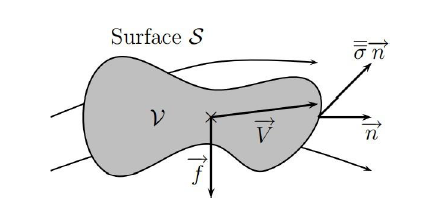
\includegraphics[width=0.6\textwidth]{figures/figure1_6.png}
    \caption{Volume de contrôle en mouvement sur lequel s'appliquent des efforts.}
    \label{fig:volume_controle_mouvement}
\end{figure}

Pour un fluide newtonien incompressible, les équations de Navier-Stokes s'écrivent sous forme vectorielle :

\begin{equation}
\rho \left( \frac{\partial \vec{V}}{\partial t} + (\vec{V} \cdot \nabla)\vec{V} \right) = -\nabla p + \mu \nabla^2 \vec{V} + \rho \vec{f}
\label{eq:navier_stokes}
\end{equation}

où les termes non encore définis précédemment sont :
\begin{itemize}
    \item[--] \(p\) : la pression statique du fluide \([Pa]\)
    \item[--] \(\mu\) : la viscosité dynamique du fluide \([Pa \cdot s]\)
    \item[--] \(\vec{f}\) : le vecteur des forces de volume (par unité de masse, typiquement la pesanteur \(\vec{g}\)) \([m/s^2]\)
    \item[--] \(\nabla p\) : le gradient de pression (force de pression par unité de volume)
    \item[--] \(\mu \nabla^2 \vec{V}\) : le terme de diffusion visqueuse (forces visqueuses par unité de volume)
\end{itemize}

Cette équation comporte deux termes fondamentaux :
\begin{itemize}
    \item Le \textbf{terme de convection} \( (\vec{V} \cdot \nabla)\vec{V} \), source de non-linéarité et de complexité. \item Le \textbf{terme de diffusion} \( \mu \nabla^2 \vec{V} \), représentant les interactions moléculaires dissipatives \cite{white2015fluid}. \end{itemize}

Les équations \eqref{eq:continuite_incompressible} et \eqref{eq:navier_stokes} forment un système de quatre équations aux dérivées partielles pour quatre inconnues (pression $p$ et les trois composantes de vitesse). Bien que mathématiquement bien posé, ce système ne possède pas de solution analytique générale en raison de sa non-linéarité \cite{kundu2015fluid}.

\section{Avantages de la CFD par rapport aux études expérimentales}
\label{sec:avantages_cfd}

Les récents progrès de la CFD en font un outil intéressant surtout en termes de coûts et de temps par rapport aux études expérimentales, dans un grand nombre de domaines de l'ingénierie, que ce soit dans l'industrie ou au niveau académique \cite{wendt2009computational}. Les différents avantages de la CFD par rapport aux essais expérimentaux en laboratoire sont résumés dans le tableau ci-dessous : \cite{roychowdhury2020computational}

\begin{table}[H]
    \centering
    \caption{Comparaison entre la CFD et les études expérimentales}
    \label{tab:comparaison_cfd_exp}
    \begin{tabular}{|l|c|c|}
        \hline
        \textbf{Critère} & \textbf{CFD} & \textbf{Études Expérimentales} \\
        \hline
        Coûts & Relativement bon marché & Cher \\
        \hline
        Temps & Court & Long \\
        \hline
        Échelles & Toutes (modèle réel possible) & Petites/Moyennes (modèles réduits) \\
        \hline
        Informations & Accès à toutes les variables en tout point & Limitée aux points de mesure \\
        \hline
        Répétabilité & Sans limite et parfaitement contrôlable & Difficile à cause des incertitudes \\
        \hline
        Sécurité & Très sécuritaire & Peut-être dangereux \\
        \hline
        Analyse de scénarios & Très simple et rapide & Lourd et coûteux \\
        \hline
    \end{tabular}
\end{table}

\section{Conclusion}
\label{sec:conclusion_chap1}

Ce premier chapitre a établi les fondements théoriques de la mécanique des fluides numérique, en présentant les équations de conservation qui constituent le socle de toute simulation CFD. La compréhension de ces équations est essentielle pour appréhender les défis liés à la modélisation des écoulements, notamment le caractère non-linéaire des équations de Navier-Stokes qui rend leur résolution analytique impossible dans le cas général. Cette situation justifie pleinement le recours aux méthodes numériques développées dans les chapitres suivants.